\let\negmedspace\undefined
\let\negthickspace\undefined
\documentclass[journal]{IEEEtran}
\usepackage[a5paper, margin=10mm, onecolumn]{geometry}
%\usepackage{lmodern} % Ensure lmodern is loaded for pdflatex
\usepackage{tfrupee} % Include tfrupee package

\setlength{\headheight}{1cm} % Set the height of the header box
\setlength{\headsep}{0mm}     % Set the distance between the header box and the top of the text

\usepackage{gvv-book}
\usepackage{gvv}
\usepackage{cite}
\usepackage{amsmath,amssymb,amsfonts,amsthm}
\usepackage{algorithmic}
\usepackage{graphicx}
\usepackage{textcomp}
\usepackage{xcolor}
\usepackage{txfonts}
\usepackage{listings}
\usepackage{enumitem}
\usepackage{mathtools}
\usepackage{gensymb}
\usepackage{comment}
\usepackage[breaklinks=true]{hyperref}
\usepackage{tkz-euclide} 
\usepackage{listings}
% \usepackage{gvv}                                        
\def\inputGnumericTable{}                                 
\usepackage[latin1]{inputenc}                                
\usepackage{color}                                            
\usepackage{array}                                            
\usepackage{longtable}                                       
\usepackage{calc}                                             
\usepackage{multirow}                                         
\usepackage{hhline}                                           
\usepackage{ifthen}                                           
\usepackage{lscape}
\begin{document}

\bibliographystyle{IEEEtran}
\vspace{3cm}

\title{8.2.27}
\author{EE25BTECH11060 - V.Namaswi}
% \maketitle
% \newpage
% \bigskip
{\let\newpage\relax\maketitle}
\renewcommand{\thefigure}{\theenumi}
\renewcommand{\thetable}{\theenumi}
\setlength{\intextsep}{10pt} % Space between text and floats
\textbf{Question}\\Find Equation of curve whose Focus is $\brak{0,-3}$ and Directrix y=3\\
\textbf{Solution}\\
General Equation of a conic is given by\\
\begin{align}
\Vec{x}^\top \Vec{V} \Vec{x} +2 \Vec{u}^\top \Vec{x}+f=0
\end{align}
where
\begin{align}
\Vec{V}=||\Vec{n}||^2 \Vec{I} -e^2  \Vec{n} \Vec{n} ^\top \\
\Vec{u}=ce^2\Vec{n}-||\Vec{n}||^2 \Vec{F}\\
f=||\Vec{n}||^2 ||\Vec{F}||^2 -c^2 e^2
\end{align}
Given,
\begin{align*}
    e=1  \quad 
    \Vec{F}=\begin{pmatrix}
        0 \\ -3
    \end{pmatrix}\\
    \Vec{n}=\begin{pmatrix}
        0 \\ 1
    \end{pmatrix}  \quad 
    c = 3
\end{align*}
From given equations,
\begin{align}
    \Vec{V}=\begin{pmatrix}
        1 & 0  \\
        0 & 1
    \end{pmatrix}-\begin{pmatrix}
        1 & 0
    \end{pmatrix}\begin{pmatrix}
        1 \\  0
    \end{pmatrix}\\
   \Vec{V} =\begin{pmatrix}
        1  & 0 \\ 0 & 0
    \end{pmatrix}\\
    \Vec{u}=3 \begin{pmatrix}
        0 \\ 1
    \end{pmatrix}-\begin{pmatrix}
        0  \\ -3
    \end{pmatrix}\\
   \Vec{u} =\begin{pmatrix}
        0 \\ 6
    \end{pmatrix}\\
    f=9-9 =0 
\end{align}
From equation 1,
\begin{align}
    \Vec{x}^\top \begin{pmatrix}
        1 & 0 \\ 0 & 0
    \end{pmatrix} \Vec{x} + 2 \begin{pmatrix}
        0 \\ 6
    \end{pmatrix} ^ \top \Vec{x} =0 
\end{align}
\begin{align}
\centering
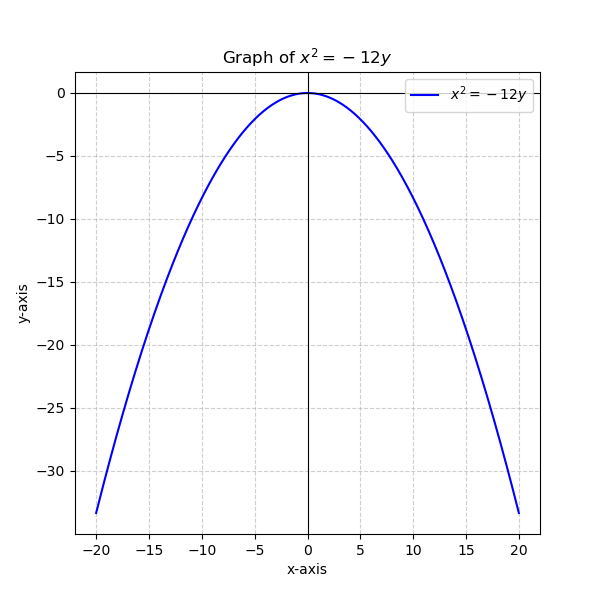
\includegraphics[width=\columnwidth, height=0.8\textheight, keepaspectratio]{figs/Figure_14.png}       
\end{align}
\end{document}